
\section{Drug Discovery Productivity Challenges}

The goal of pharmaceutical sciences is to identify and market safe and efficacious drugs. Toxicity is a large contributor to drug candidate attrition in drug development. Inhibition of enzymes in the cytochrome P450 superfamily is a major source of toxicity in human and animal models because of their role in first pass metabolism. If a compound inhibits cytochrome P450 it is likely to lead to toxic effects when first pass metabolism fails to clear other therapeutic compounds or alters their pharmacokinetics. Because the discovery and development of a each new pharamceutical drug requires more than a billion dollars across an average of 12 years, it would be useful to know whether a compound of interest inhibits cytochrome P450s as early as possible.

The Cytochrome P450 superfamily is large and varied. Different isozymes metabolize different substrates. Even within and between individuals pharmacokinetic and pharmacodynamic variability can be high for reasons not entirely characterized. Designing assays for every isozyme and SNP variant and running them against every compound of interest as a general strategy is cost prohibitive. This project was designed to test the predictive power of computational methods for cytochrome P450 inhibition potential based simply on knowledge of chemical structure.

There has been an upward trend in drug development costs for three decades for a variety of reasons. Integrated computational approaches have been proposed as one way to control costs in pharamceutical research and development. \cite{Visser2014} The foundational skills demonstrated in this thesis are needed to pursue a systems approach to drug development that industry has recently turned toward as a way to boost R\&D productivity. \cite{Berg2014} It is also part of the larger project of \textit{in silico} drug-development, which is attempting to reduce reliance on exploratory \textit{in vivo} and clinical drug testing and increase the number of effecive treatments for patients while decreasing the amount of time to develop them.

%Math is the new microscope \cite{Cohen2004}

An approach to associating compound structure with bioactivity that goes back at least to Hansch \cite{Hansch1964} has progressed under the moniker of Quantitative Structure Activity Relationship (QSAR). QSAR started with direct measures of chemical compounds and later derived features and used them to then build expert systems or statistical models that tried to predict biological activity. During those same decades, the field of machine learning emerged; using computation in an analogous and more general way -- to associate features with results, inputs with outputs. Machine learning can be thought of as using algorithms to figure out how to perform important tasks by generalizing from examples. These algorithms are of course usually laborious, which necessitates their execution by computer.

Statistical machine learning builds upon the peer prediction of machine learning. It also allows for prediction but focuses more on models and methods that can be used by scientists and engineers. \cite{James2013} Further extension of statistical learning to the pharmaceutical sciences can lead to important contributions to systems pharmacology. Or rather statitical learning methods are an important precursor to the needs of systems biology and systems pharmacology modeling.

This project compares different techniques for Cytochrome P450 inhibition prediction in the framework of statistical learning. To demonstrate generality and apllicability to the pharmaceutical sciences the five isozymes of Cytochrome P450 that are involved in metabolism of 90\% of all therapeutic drugs (CYPs 1A2, 2C9, 2C19, 2D6 and 3A4) are the subject of this study.

Because replicability is one of the main principles of the scientific method, as much as possible, the code and data used in this study is publicly available and source controlled. Reproducibility as a practice is a habit, and a good one to get into. Every attempt was made to make the materials and methods for this project reproducible in a completely automated way to allow for validation of results and extension of the work.

\section{Cytochrome P450 Superfamily}

One of the largest and most functionally diverse protein superfamilies is the cytochrome P450 family of hemoproteins. From bacteria to humans, the functional breadth of cytochrome P450 activity is far ranging. At the latest count there were significantly more than 2000 identified cytochrome P450 genomic and cDNA sequences that have been divided into a total of 265 different families. \cite{Danielson2002} Cytochromes P450 appear in every kingdom from bacteria to higher eukaryotes. Multiple cytochrome P450 genes can be expressed simultaneously as different isozymes and the number of genes per species is highly variable with a tendency for higher eukaryotes to possess more. The cytochromes P450 (CYPs) constitute the major enzyme family capable of catalyzing the oxidative biotransformation of most drugs and other lipophilic xenobiotics and are therefore of particular relevance for clinical pharmacology. This central role that these ubiquitous proteins play as phase I enzymes in human drug metabolism makes them very important to the pharmaceutical industry.

\begin{figure}[H]
  \caption{Ribbon Diagram of CYP1A2}
  \centering
   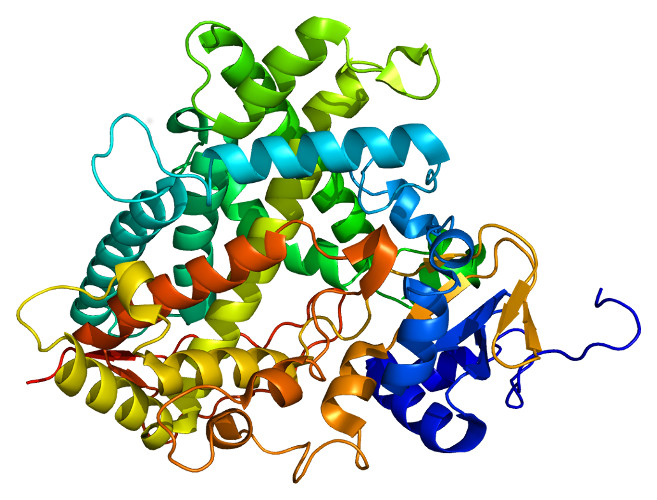
\includegraphics[width=1\textwidth]{../img/CYP1A2_PDB.jpg}
\end{figure}

\begin{figure}[h,t]
  \caption{Ribbon Diagram of CYP3A4 with heme center}
  \centering
   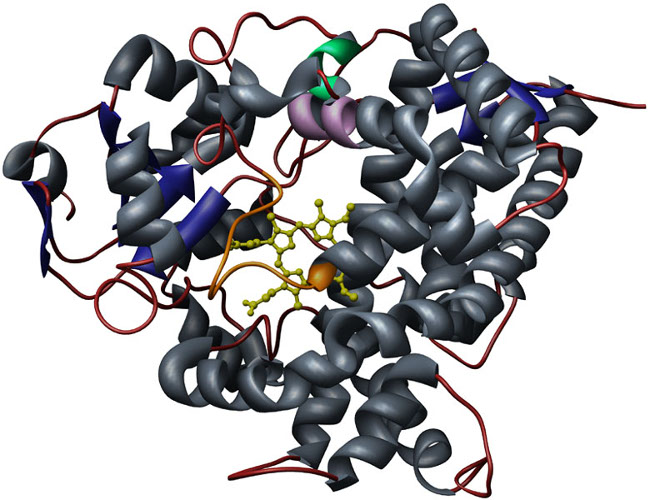
\includegraphics[width=1\textwidth]{../img/CYP3A4_heme.jpg}
\end{figure}


CYP families are classified based on pairwise amino acid sequence identity among individual members. Families CYP 1-3 are involved in phase I metabolism of human drugs and xenobiotic compounds, whereas other CYP families (CYP 4, 11, 17, 17 and 21) are involved in the metabolism of endogenous compounds such as fatty acids, steroids, eicosanoids, bile acids and fat soluble vitamins\cite{Singh2011}

\begin{figure}[h,t]
  \caption{Mecahism of Action of Cytochrome P450 Catalytic Heme Group}
  \centering
   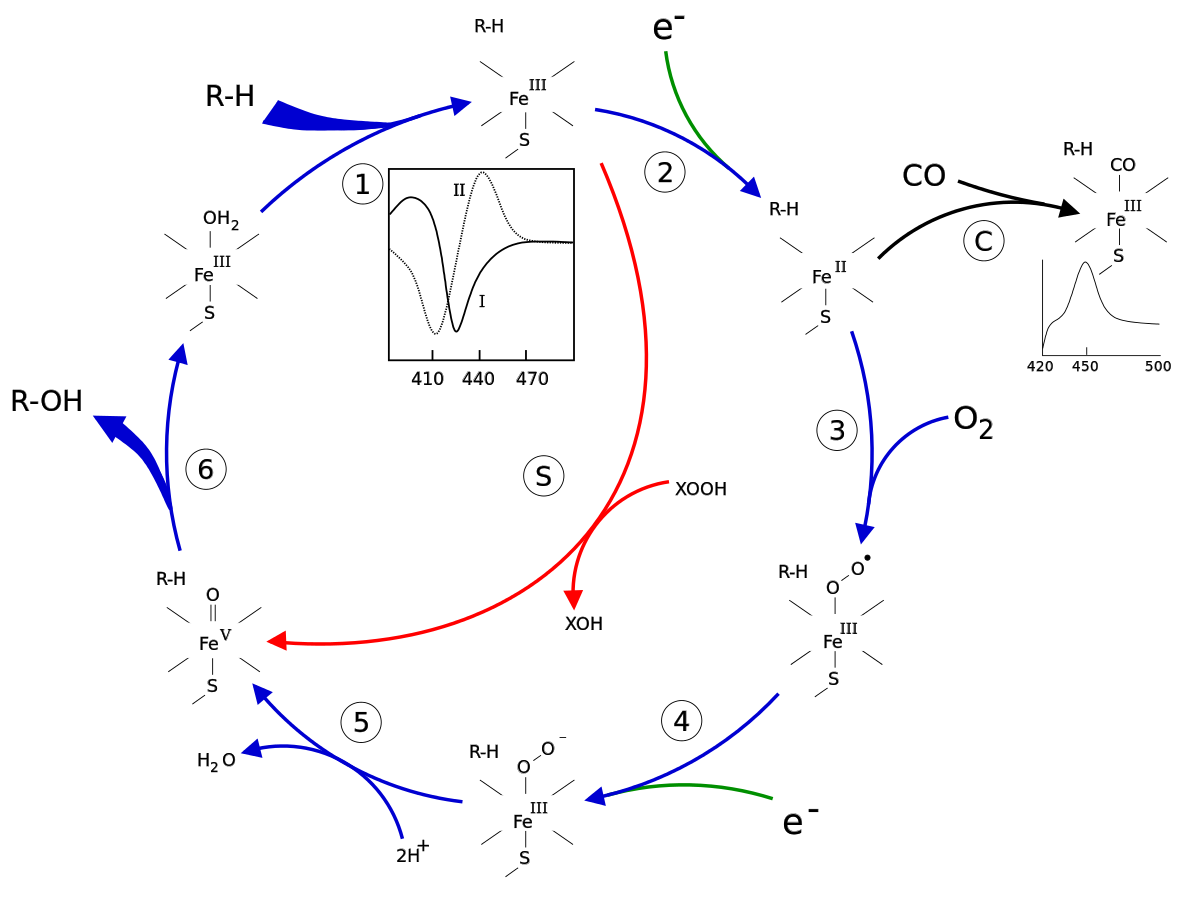
\includegraphics[width=1\textwidth]{../img/P450MOA.png}
\end{figure}

There is a considerable substrate overlap between enzymes of this superfamily. Being broadly specific with respect to their substrates, CYPs are therefore susceptible to inhibition by a large variety of chemical compounds. It follows that the CYP enzymes that are involved in the oxidative metabolism of drugs play a major part in the activation and elimination of therapeutic drug molecules. CYP inhibition leading to decreased elimination and/or changed metabolic pathways of other substrates is a major cause of adverse drug-drug interactions. \cite{Lapins2013} So adverse side effects of drug-drug interactions are an important area of inquiry, especially during the research phase of drug discovery.


\section{Early Compound Profiling \textit{In Silico}}

Drug discovery is a multi-parameter optimization process in which compounds are optimized for interaction with their target while minimizing off-target activities. \cite{Zlokarnik2005} In the normal course of taking a compound from hit to lead to drug candidate adding drug-like properties may minimize the risk of making potent and target-class selective compounds that are biologically inaccessible but at the same time does little to address the combinatorical complexities of specific drug-drug interactions due to off-target effects.

%Project teams often pursue a parallel optimization approach in which multiple scaffolds are explored along multiple axes, including potency, selectivity, physicochemical properties and absorption, distribution, metabolism, excretion and toxicity (ADME­Tox) parameters(1-6)\cite{Zlokarnik2005}

Because of the complex nature of toxicity, safety prediction is considered more challenging than efficacy prediction. Toxicity mechanisms may be unknown or poorly characterized in higher organisms, and similar pathways and targets may be associated with different toxicities and adverse events. Toxicity prediction must also encompass a number of complex interactions and remain alert to the possibility of finding the unexpected. For instance, toxicities could result from on-target effects due to incomplete knowledge or inadequate target validation, or from off-target effects mediated via unknown molecules and mechanisms, or even from genetic variation or comorbidities in any of the previously mentioned pathways. \cite{Kruhlak2012}

Techniques for high-throughput \textit{in vitro} screening of CYP inhibition have been developed and implemented broadly in drug discovery pipelines across pharmaceutical companies and research institutions, resulting in the generation of large datasets. Some of this accumulation of data has been released through academic research initiatives (e.g. PubChem Bioassays AID 410 and 1851). These collections enable development of structure-activity relationship models for \textit{in silico} prediction of CYP inhibition by a much larger pool of researchers than those who designed and carried out the assays.

The promise of \textit{in silico} screening that remains very appealing is that, with a steady increase in computing power, screening cost could become negligible. The hope is that virtual compounds could be screened for CYP liabilities in order to realize savings and reduce the number of candidates with questionable prospects that would otherwise be synthesized. \cite{Zlokarnik2005} Acheiving this would also turn the costly animal toxicity test phase of preclinical research into a validation step rather than a screening step.

%As a major advance, the crystal structures of several human CYP isozymes have been solved. These structures provide more accurate geometries of the enzymes’ active sites and should lead to better representations than previous homology models that were based on crystal structures of soluble bacterial enzymes.\cite{Zlokarnik2005}

% but share the disadvantage that they are not implemented as publicly available services.\cite{Lapins2013}

%Another deficiency of these models (except Cheng) is the use of molecular descriptors that are calculated by commercial software packages, which does not allow implementation of the models in free, open source software.\cite{Lapins2013}

In order to generate the necessary data, many high-throughput technologies are now available to detect P450 inhibitors. High-throughput screening data can be used to guide medicinal chemists away from these interactions in an early stage. In certain cases it might also identify the inhibition issue by targeted modification of the CYP interacting functionality. To be generally useful, P450 inhibition screens need to be calibrated against standard methods and preferably also tested with a large set of drugs, for which human drug-drug interaction outcome is known. \cite{Zlokarnik2005} This should decrease the number of withdrawls of novel drugs from the market due to inhibition of major P450 isozymes.

The ability to predict clinical safety based on chemical structures is also becoming an increasingly important part of regulatory decision-making. QSAR models are currently used by in industry and by regulators to evaluate safety concerns and possible nonclinical effects of a drug when adequate safety data is absent or inconclusive.\cite{Kruhlak2012}

The United States is about to become the last country to accept QSAR in the drug approval process. The drafting of International Committee on Harmonization (ICH) M7 guideline can be viewed as setting a precedent for possible future, broader regulatory applications of QSAR modeling. ICH M7, will for the first time specify that -- under very specific conditions -- the results of QSAR computational toxicology predicitions will be considered sufficient for genotoxic contaminants of pharmaceuticals under consideration and thereby eliminate the need for laboratory testing. \cite{Kruhlak2012}


\section{Quantitative Structure-Activity Relationship}

Quantitative structure-activity realtionship (QSAR) modeling is generally accepted as the construction of predictive models of biological activities as a function of structural and molecular information of a compound or compound library. \cite{Nantasenamat2009}

QSAR models describe the correlation between molecular features and activity at a given end point of interest. There have also been attempts to make structure activity models (SAR) constructed by using human expert knowledge (“expert rule-based”), but QSAR models are typically defined as those that use statistical methods to analyze the mathematical correlations between molecular features and activity. 

A QSAR model that defines the mathematical relationships between descriptors and biological activities of know molecules, differs from receptor binding-based efficacy prediction which takes into account binding site characteristics as well as molecular docking analysis. In contrast to QSAR, receptor-binding methods attempt to predict drug efficacy based on known mechanisms of action and medicinal chemistry by individually studying molecular interactions between a drug and targets/receptors. \cite{Kruhlak2012}

It follows from the 'similarity principle' that new and untested compounds possessing similar molecular features as known compounds are assumed to possess similar activities and properties. In this way, QSAR models can make it possible to predict the biological activities of a given compound as a function of its molecular structure. Several successful models have been published over the years which encompass a wide span of biological and physicochemical properties.

Applied QSAR, as described above, has typically been used for drug discovery and development but has also been used to correlate molecular information with other physiochemical properties. This later approach is termed quantitative structure-property relationship (QSPR). Derived molecular parameters can account for hydrophobicity, topology, electronic properties, and steric effects. These characteristics of compounds can either be determined empirically through experimentation or theoretically via computational chemistry as needed. \cite{Nantasenamat2009} The parameters derived from compound structure are refered to as molecular descriptors.

%A given compilation of data sets is then subjected to data pre­processing and data modeling through the use of statistical and/or machine learning techniques.\cite{Nantasenamat2009}

%Drug discovery has often evolved from serendipitous and fortuitous findings, for example, the discovery of penicillin by Alexander Fleming in 1928 triggered the antibiotic revolution... If not by chance, such discoveries may be achieved through random systematic experimentation or chemical intuition where combinatorial libraries are synthesized and then screened for potent activities. A potentially more lucrative approach is to rationally design drugs using computer­aided tools via molecular modeling, simulation, and virtual screening for the purpose of identifying promising candidates prior to synthesis.\cite{Nantasenamat2009}

%Data understanding is equivalent or can be achieved through exploratory data analysis which often starts with simple observation of the data matrix particularly the variables (also known as attributes or fields), its corresponding data types, and the data samples (also called records). As applied to the QSAR discipline, variables represent molecular descriptors; data samples represent each unique compound; data types refer to the characteristics or the kinds of data the particular value is represented as, which is essentially qualitative or quantitative in nature. Qualitative data types are interpreted as categorical labels while quantitative data types are amenable to arithmetic operations.\cite{Nantasenamat2009}

\subsubsection{Molecular Descriptors}
Molecular descriptors can be thought of as the mathematical representation of essential information of a molecule in terms of its own physiochemical properties. Depending on the needs of the analysis, properties considered can be electronic, geometric, hydrophobic, constitutional, lipophilic, steric, solubility, quantum chemical, or topological. From a practical viewpoint, molecular descriptors are chemical information that is encoded within the molecular structures. \cite{Nantasenamat2009}

%The activities and properties that can be modeled by QSAR/QSPR are dependent variables of the QSAR model. These dependent variables are assumed to be influenced by the independent variables which are the molecular descriptors. A variety of biological and chemical properties have been modeled using the QSAR approach, such parameters are summarized as: Biological Properties Bioconcentration, biodegradation, carcinogenicity, drug metabolism and clearance, inhibitor constant, mutagenicity, permeability across blood brain barrier or skin, pharmacokinetics, receptor binding. Chemical Properties boiling point, chromatographic retention time, dielectric constant, diffusion coefficient, dissociation constant, melting point, reactivity, solubility, stability, thermodynamic properties, viscosity. \cite{Nantasenamat2009}

Molecular features can be either experimentally measured or calculated values. They come in the form of simple physiochemical properties such as logP or logarithmic acid dissociation constant (pKa), numerical representaions of substructure fragments, or purely mathematical descriptors. Mathematical descriptors are chemical structural features represented in numerical form, and range from simple atom counts to the product of complex equations that describe electron distribution across a molecule. \cite{Kruhlak2012}

Molecular descriptors as predictors in QSAR modeling are typically less precise than the “lock and key” relationships that underpin the docking approach to computer-aided drug design. The basic assumption in QSAR modeling is that similar molecules exhibit similar biological activity so that physiochemical properties and/or structural properties of a molecule encoded as molecular descriptors can be used to predict the biological activity of structurally related compounds with some degree of confidence.

\subsubsection{Modeling}
QSAR models can be described as global or local. Global models incorporate chemicals with a range of molecular features acting across the spectrum of chemical pathways, whereas local models are highly focused on a single chemical class and end point. Although local models generally have much higher accuracy, their narrow domain of applicability renders them impractical in most regulatory environments where predictions need to be made across a variety of molecules including active pharmaceutical ingredients, metabolites, reagents, and synthetic intermediates. \cite{Kruhlak2012}

The construction of QSAR models typically follows two main steps:
\begin{itemize}
\item Description of molecular structure with derivation of descriptors
\item Multivariate analysis correlating molecular descriptors with observed activities. 
\end{itemize}
Additional intermediate steps are also crucial for sucessful development of such QSAR models and include data preprocessing and statistical evaluation. \cite{Nantasenamat2009}

\begin{figure}[h,t]
  \caption{Typical QSAR Workflow}
  \centering
  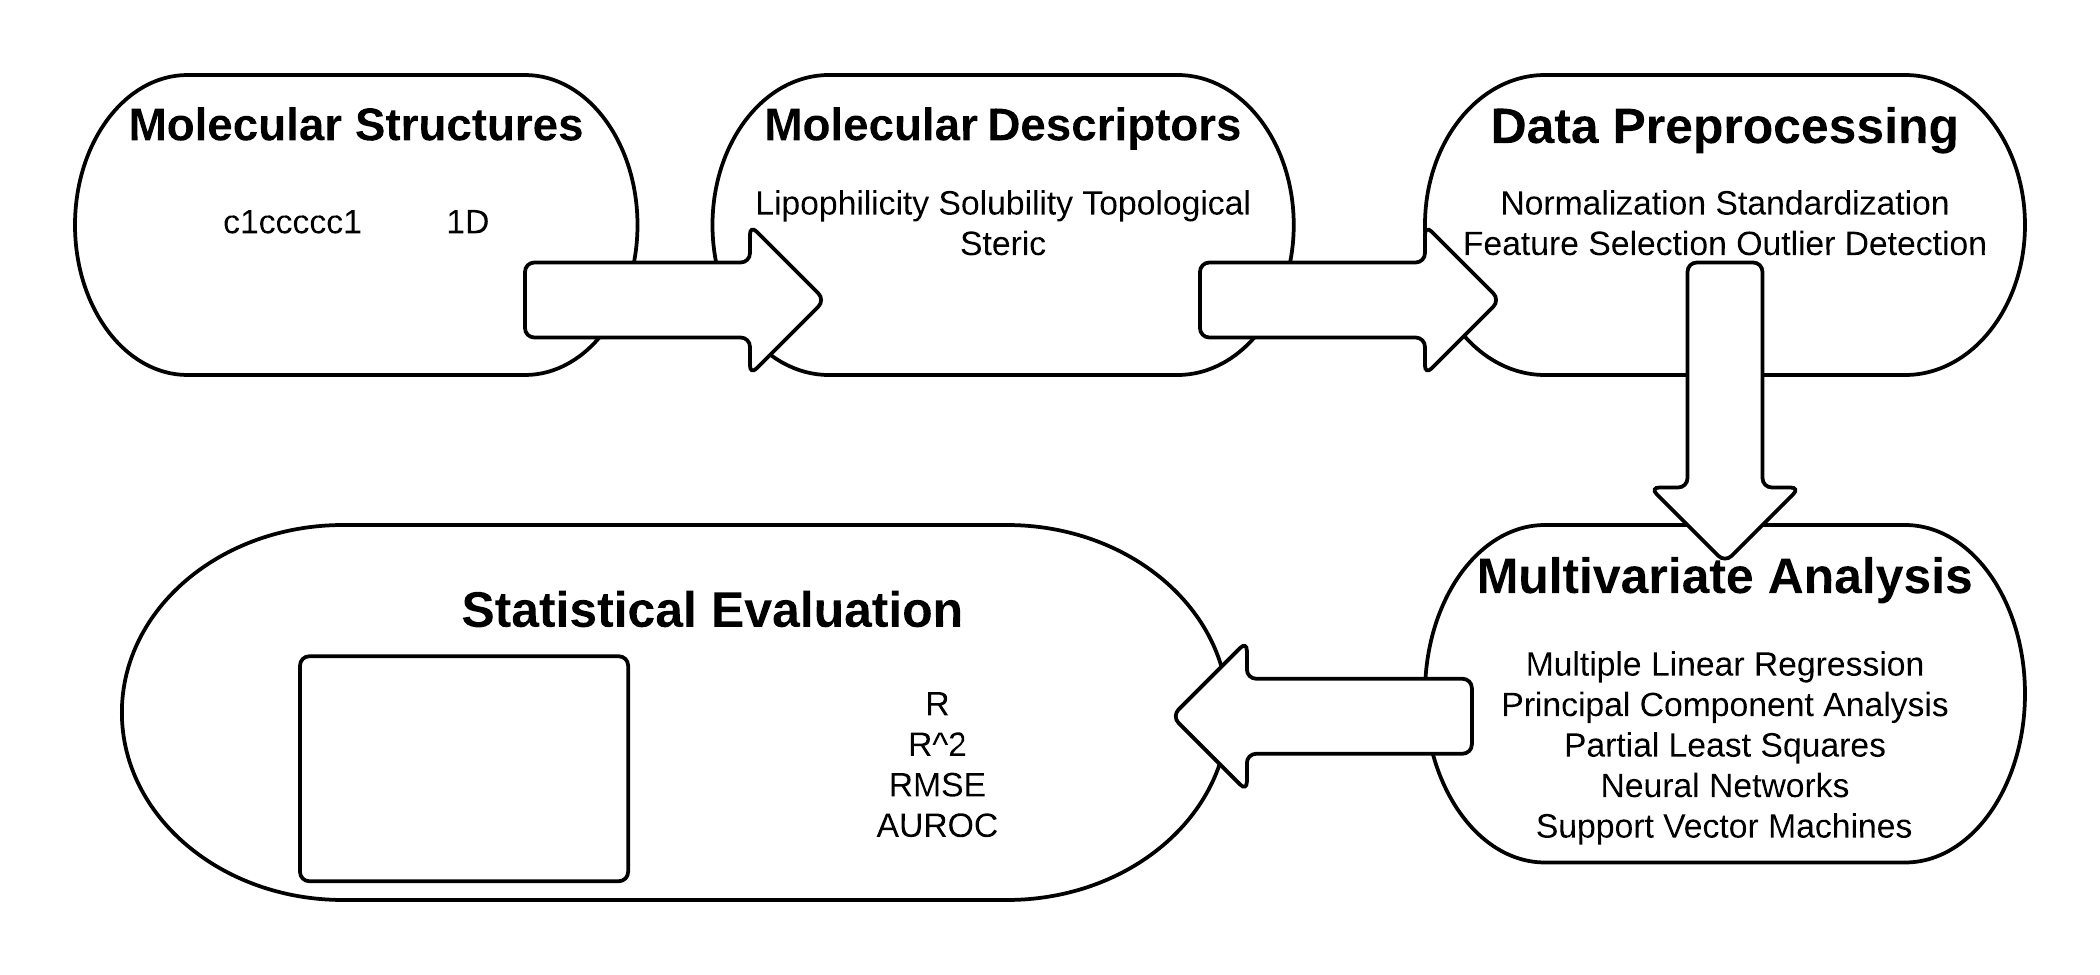
\includegraphics[width=1\textwidth]{../img/Typical_QSAR_Process.png}
\end{figure}

A typical QSAR workflow treats chemical structure management, descriptor calculation, and statistical analyses as separate steps that are often performed by non-integrated software packages. This can lead to low throughput and even the lack of possibility of performing predictions for new compounds or updating the models when new data become available, depending on the workflow.

According to Kruhlak, et al., the successful development of a QSAR model for safety prediction requires a sufficient amount of high-quality data, the appropriate selection of descriptors, the availability of one or more suitable statistical or mathematical models and an effective training and validation strategy.
\cite{Kruhlak2012}
%Creating structure-activity models for one CYP isozyme at a time may be a suboptimal approach since the inhibition profiles of CYPs largely overlap. A more general technique is proteochemometrics (PCM, a modelling technology that 'Sweden' introduced to study similarities and differences in molecular interaction mechanisms of groups of related proteins.\cite{Lapins2013}

%PCM creates unified models for multiple proteins interacting with multiple ligands by correlating the interaction data to descriptors of both sets of interacting entities.\cite{Lapins2013}

%In this study they aimed to create a unified PCM model for CYPs suited for drug profiling using free, open­access software and make the model publicly available for predictions.\cite{Lapins2013}

\section{Statistical Machine Learning}

Machine learning algorithms figure out how to perform important tasks by generalizing from examples. A concise definition of statistics is as the applied science that constructs and studies techniques for data analysis (Jan de Leeuw) Statistical learning refers to a set of approaches for estimating a function that describes a dataset as a precursor for prediction or inference. \cite{James2013} Statistical machine learning constructs that function by generalizing from examples, i.e. data.

Leo Breiman wrote a landmark paper that documented the beginnings of this approach. He said 
\begin{quote}
'There are two cultures in the use of statistical modeling to reach conclusions from data. One assumes that the data are genereated by a given stochastic data model. The other uses algorithmic models and treats the data mechanisms as unknown' \cite{Breiman2001}
\end{quote} He goes on to claim that the statistical community had traditionally prefered the first view.

Classification is a well understood area of machine learning. A classifier takes a system of inputs, typically a vector of discrete and/or continuous feature values and then outputs a single discrete value, the class. \cite{Domingos2012}

The current state of machine learning is fundamentally a subset of optimization and has found its biggest successes in fields where there are far more variables than parameters. The ultimate goal of machine learning in these cases is to generalize beyond examples in the training set, because no matter how much data there is, it is unlikely that those exact examples will be seen again at test time. \cite{Domingos2012} 

%Everyone knows about overfitting, but it comes in many forms that are not immediately obvious. One way to understand overfitting is by decomposing generalization error into bias and variance.\cite{Domingos2012}

In the context of QSAR then, with enough prior knowledge and sound assay results, machine learning may be a practical approach to fill in the gaps of clinical knowledge for any relevant CYP isozyme when queried against any untested compound of interest so long as the compound structure is known.

This is a wider view than traditionally encountered in most applied science education where simple hypothesis testing predominates. Opening up the field of data analysis like this brings opportunity for exploration but also new concerns, such as the 'curse of dimensionality', 'degrees of freedom of the analyst', 'black box algorithms', difficulty of bias estimation and the 'no free lunch theorem'. \cite{Boulesteix2014}


%\subsubsection*{Learning = representation + evaluation + optimization}

%\begin{itemize}
%\item Representation = A classifier must be represented in some formal language that the computer can handle. A representation for the learner is tantamount to choosing the set of classifiers that it can possibly learn. This set is called the hypothesis space.

%\item Evaluation = Often called the evaluation function, objective function, or scoring function - distinguishes good from bad classifiers.

%\item Optimization = a method to search among classifiers for the highest scoring one.

%\end{itemize}

%Most textbooks are organized by representation, but the other components -- evaluation and optimization -- are equally important.\cite{Domingos2012}

\section{Sources of Data for Learning}

Systems biology research encompasses the generation of high-throughput datasets of system components (omics data), experimental methods of analysis and data integration, as well as the development and application of network approaches and computationally derived models. \cite{Berg2014} In pharmaceutical research, systems biology efforts are directed towards the identification of drug targets, the development of novel therapeutics and new indications for existing drugs.

Omics tools, developed over the past several decades, can provide global information on the levels and dynamic changes in cellular and tissue components at specific time points insamples from cell-based assays, precinical animal models or human studies. Omics data sets derived from transcriptomics, proteomics, and metabolomics are being used and integrated with each other as well as genomics information and other data types to construct models of cell signaling, pathway and disease networks to identify new targets as well as to help better understand and predict drug action in vivo.

Studies tend to be compound-centric, concerned with the identification and characterization of small molecules or biologics that selectively inhibit (or activate) specific molecular targets or pathway mechanisms. These kinds of studies are particularly useful to drug discovery research as the attempt to work out related drug mechanisms of action. They also support secondary drug development goals, such as clinical indication selection and patient stratification. \cite{Berg2014}

% ""In addition to experimentally derived data sets, there is a wealth of literature information and accumulated knowledge that can be incorporated by converting to some type of formal representation. This is accomplished through the use of a defined ontology by expert curation and/or natural language processing(NLP) - based methods into a series of semantic statements.""(Berg2014)
\begin{quote}
The ultimate goal of systems biology in this context is an understanding of physiology and disease across the multiple hierarchical levels of organization, from chemical and molecular interactions to pathways and pathway networks, at the cell-cell and tissue level, organs and organ systems and, ultimately, to the functioning of the whole organism.
\end{quote}


\section{Reproducibility}

Several recent publication has highlighted the negative impact of irreproducible biomedical research, such as the group from Bayer that claimed they had to halt two-thirds of their research efforts in 2011 \cite{Prinz2011} and the group from Amgen that reported only an 11\% success rate in trying to replicate the effects of major cancer drug findings. \cite{Begley2012} In the latter case we don't even know which drugs were tested because those findings are not public either. Information generation can happen far faster and is much more common than data analysis and knowledge creation in the biological sciences.

One of the issues to overcome in this area include the need for more biologists trained in quantitative and statistical methods for analyzing large data sets are the open release of findings and experimental protocols. 

Science conducted in an open fashion confers the following benefits

\begin{itemize}

\item Reproducibility of experiments allows other researchers to use the exact methods to calculate the relations between biological data.

\item Faster development of disease models and therapeutic treatments due to the reuse of existing knowledge. Projects can be built upon existing results more easily or extend the research in directions unanticipated by the original team. First-pass results can be subject to new analysis, and a second look at compounds with interesting side effects can lead to serendipidous discoverys

\item Increased quality as a result of having more researchers studying the same topic to provide a layer of assurance that errors will not propagate.

\item Long-term availability of data and code. If these resources are not tied to businesses or patents, then they can be posted to multiple repositories to ensure that they are available in the future.
\cite{Prlic2012}

\end{itemize}

New research findings, supporting data and methods should, therefore, be made publicly available for independent verification and replication in order not to delay medical advances.



\section{Aims}
The aim of this project is to build QSAR models that quantify the risk of off-target effects for candidate molecules by building statistical machine learning models that make binary classification as inhibitors or non-inhibitors of Cytochrome P450 of compounds based on their structure.

We will compare a well accepted, commercial method of binary classification with a three open source implementations of QSAR model building according to the following plan:

\begin{itemize}

\item Build Binary QSAR models in the Molecular Operating Environment (MOE).

\item Develop and implement comparable methods in open source software.

\item Evaluate and compare results from all models.

\item Perform this analysis as reproducible research.

\end{itemize}
